\chapter{Cálculo de intersecciones rayo-superficie mediante métodos iterativos}

${ }$\\

En Ray-Marching para calcular las intersecciones de los rayos con una superficie dada en su ecuación implícita
${ }$\\
\[
	F(x,y,z) = 0,
\]
${ }$\\
vamos a usar el método de Newton-Raphson y Regula-Falsi de forma combinada ya que cada uno tiene unas ventajas e inconvenientes que justifican el uso de ambos. Mientras Newton-Raphson no garantiza que se llegue a una aproximación de la solución y la sucesión que genera puede divergir como se verá mas adelante, el método de Regula-Falsi asegura la convergencia de la solución. Sin embargo, el método de Newton-Raphson converge mas rápido que Regula-Falsi.
${ }$\\

Para programar esta segunda parte tuve que hacer algunos cambios y mejoras en el código que ya tenía, entre las modificaciones se puede encontrar una nueva clase llamada $Rayo$ con la se representarán los rayos para hacer la lectura del código un poco mas intuitiva. Las modificaciones son las que se muestran a continuación:
${ }$\\

\begin{lstlisting}[style=Consola]
class Rayo{
	
private :
	
	Tupla3f origen, direccion;
	
public :
	
	Rayo(Tupla3f o, Tupla3f d);
	Tupla3f puntoRayo(double t);
	Tupla3f getOrigen();
	Tupla3f getDireccion();
};
	
Rayo::Rayo(Tupla3f o, Tupla3f d){

	origen = o;
	direccion = d;
}
	
Tupla3f Rayo::puntoRayo(double t){

	return origen + t*direccion;
}
	
Tupla3f Rayo::getOrigen(){

	return origen;
}
	
Tupla3f Rayo::getDireccion(){

	return direccion;
}
\end{lstlisting}
${ }$\\



Aquí, se puede observar que la función $derivada$ necesaria para el cálculo del siguiente valor de la sucesión de Newton-Raphson se calcula haciendo una aproximación mediante la fórmula:
${ }$\\

$$ f'(x) = \lim_{h \to 0} \frac{f(x+h) - f(x)}{h} $$
${ }$\\


\begin{lstlisting}[style=Consola]
class Superficie {

private :

	Tupla3f color;

	void intervaloInicial(Superficie &sup, Rayo rayo, double &t1, double &t2);
	double RegulaFalsi(Superficie &sup, double an, double bn, Rayo rayo);
	double NewtonRaphson(Superficie &sup, double tn, Rayo rayo);
	double derivada(Rayo rayo, double t);

public :

	Superficie(Tupla3f col);
	Superficie(const Superficie &sup);
	virtual double interseccion(Superficie &sup, Rayo rayo);
	virtual Tupla3f normal(Tupla3f xyz);
	virtual Tupla3f getColor();
	virtual double funcion(Tupla3f xyz) = 0;
};

Superficie::Superficie(Tupla3f col){

	color = col;
}

Superficie::Superficie(const Superficie &sup){

	color = sup.color;
}


Tupla3f Superficie::getColor(){

	return color;
}

double Superficie::interseccion(Superficie &sup, Rayo rayo){

	double an, bn, tn;
	int num_iteraciones = 0;

	intervaloInicial(sup, rayo, an, bn);

	tn = an;

	if (sup.funcion(rayo.puntoRayo(an)) == 0) return an;
	else if (sup.funcion(rayo.puntoRayo(bn)) == 0) return bn;
	else if (an == bn) return -1;

	while (abs(sup.funcion(rayo.puntoRayo(tn))) > 0.1 && num_iteraciones < 100){
	
		tn = NewtonRaphson(sup, tn, rayo);

		if (tn < an || bn < tn) tn = RegulaFalsi(sup, an, bn, rayo);

		if (sup.funcion(rayo.puntoRayo(tn)) == 0) return tn;
		else if (sup.funcion(rayo.puntoRayo(an))*sup.funcion(rayo.puntoRayo(tn)) > 0) an = tn;
		else bn = tn;
		
		num_iteraciones++;
	}

	return tn;
}

void Superficie::intervaloInicial(Superficie &sup, Rayo rayo, double &t1, double &t2){

	t1 = 0;
	double incremento = 0.1;
	
	while ( (sup.funcion(rayo.puntoRayo(t1)) * sup.funcion(rayo.puntoRayo(t1+ incremento)) > 0) && t1 < 2) t1 = t1 + incremento;
	
	for (int i = 0; i < 3; i++){
	
		t2 = 0;
		
		while ( sup.funcion(rayo.puntoRayo(t2)) * sup.funcion(rayo.puntoRayo(t1)) > 0 && t2 < 2){
			t2 = t2 + incremento;
		}
		
		if ( sup.funcion(rayo.puntoRayo(t2)) * sup.funcion(rayo.puntoRayo(t1)) > 0 ) break;
		else incremento = incremento / 3;
	}
}

double Superficie::RegulaFalsi(Superficie &sup, double an, double bn, Rayo rayo){

	if (sup.funcion(rayo.puntoRayo(an)) == sup.funcion(rayo.puntoRayo(bn))) cout << "notANumber" << endl;
	
	return ( ( (an*sup.funcion(rayo.puntoRayo(bn))) - (bn*sup.funcion(rayo.puntoRayo(an))) ) / ( sup.funcion(rayo.puntoRayo(bn)) - sup.funcion(rayo.puntoRayo(an)) ) );
}

double Superficie::NewtonRaphson(Superficie &sup, double tn, Rayo rayo){

	return tn - (sup.funcion(rayo.puntoRayo(tn))/sup.derivada(rayo, tn));
}

Tupla3f Superficie::normal(Tupla3f xyz){

	return normalized( Tupla3f(funcion( xyz + Tupla3f(EPSILON, 0.0, 0.0) ) - funcion( xyz - Tupla3f(EPSILON, 0.0, 0.0) ), funcion( xyz + Tupla3f(0.0, EPSILON, 0.0) ) - funcion( xyz - Tupla3f(0.0, EPSILON, 0.0) ), funcion( xyz + Tupla3f(0.0, 0.0, EPSILON) ) - funcion( xyz - Tupla3f(0.0, 0.0, EPSILON) )) );
}

double Superficie::derivada(Rayo rayo, double t){

	return (funcion(rayo.puntoRayo(t + EPSILON)) + funcion(rayo.puntoRayo(t))) / EPSILON;
}
\end{lstlisting}
${ }$\\



${ }$\\
\section{Newton-Raphson}
%$\textbf{Newton-Raphson}$
${ }$\\

Como se puede ver en la Figura \ref{fig:etiq_7} el método de Newton-Raphson comienza tomando una aproximación inicial $x_0$. Para calcular el siguiente valor de la sucesión se toma la recta tangente en el punto $(x_n, f(x_n))$, la intersección de esta recta con el eje de abscisas será el siguiente valor de la sucesión, $x_{n+1}$.
${ }$\\

\begin{figure}[h]
	\begin{center}
		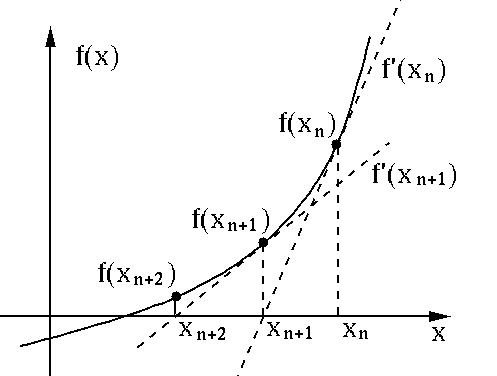
\includegraphics[width=1.0\textwidth]{imagenes/newton.png}
	\end{center}
	\caption{Construcción gráfica de la sucesión dada por el método de Newton-Raphson. Imagen tomada de \cite{CarmenS}.}
	\label{fig:etiq_7}
\end{figure}
${ }$\\

El algoritmo a seguir es el siguiente:

\begin{itemize}
	\item Paso 0 : Tomar un $x_0$ inicial.
	\item Paso 1 : $x_{n+1} = x_n - \frac{f(x_n)}{f'(x_n)}$.
	\begin{itemize}
		\item Si $f(x_{n+1}) = 0$, hemos terminado.
	\end{itemize}
\end{itemize}
${ }$\\

\begin{lstlisting}[style=Consola]

double Superficie::NewtonRaphson(Superficie &sup, double tn, Tupla3f o, Tupla3f d){

	return tn - (sup.funcion(o, d, tn)/sup.derivada(o, d, tn));
}

\end{lstlisting}
${ }$\\



Se puede observar que no siempre es posible calcular el siguiente $x_{n+1}$ ya que la derivada de la función en $x_{n}$ podría ser $0$.
${ }$\\
${ }$\\

${ }$\\
\section{Regula-Falsi}
%$\textbf{Regula-Falsi}$
${ }$\\

El algoritmo de Regula-Falsi es un refinamiento del método de bisección. Al igual que en el método de bisección partimos de un intervalo inicial $[a_0, b_0]$, teniendo $F(r(a_0))$ y $F(r(b_0))$ signos opuestos(aquí estamos considerando que F es la función implícita $F(x,y,z)$ y $r(t)$ es la ecuación del rayo). Esto nos es de utilidad ya que como dice el Teorema\ref{teo:bolzano} esto nos garantiza que hay una solución dentro de ese intervalo. Este método va calculando intervalos cada vez mas pequeños que incluyen a la solución.
${ }$\\

Como se puede ver en la Figura \ref{fig:etiq_8}, gráficamente el procedimiento toma la recta que pasa por los puntos $(a_0, F((a_0)))$ y $(b_0, F((b_0)))$ y toma el punto de intersección de esta con el eje de abscisas. El nuevo intervalo se ajustará dependiendo de que el valor de la función en este nuevo punto sea negativo o positivo poniendose en el lugar de $a_1$ o $b_1$ de tal manera que se siga cumpliendo $F(r(a_1)) \cdot F(r(b_1)) < 0$.
${ }$\\

\begin{figure}[h]
	\begin{center}
		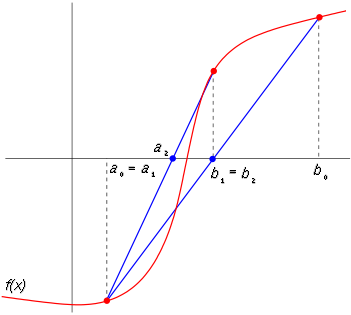
\includegraphics[width=0.8\textwidth]{imagenes/regulaF.png}
	\end{center}
	\caption{Construcción gráfica del método de Regula-Falsi. Imagen sacada de https://de.wikipedia.org/wiki/Regula\_falsi.}
	\label{fig:etiq_8}
\end{figure}
${ }$\\

\begin{teorema}\label{teo:bolzano}
	$\textbf{(de los ceros de Bolzano)}$ Sea una función continua $f : [a,b] \to \mathbb{R}$ tal que $f(a) \cdot f(b) < 0$, entonces existe al menos un $s \in (a,b)$ tal que $f(s) = 0$.
\end{teorema}
${ }$\\



El algoritmo de Regula-Falsi es el siguiente:

\begin{itemize}
	\item Paso 0 : Tomar un $a_0$ y $b_0$ iniciales.
	\item Paso 1 : $m_n = \frac{a_n f(b_n) - b_n f(a_n)}{f(b_n) - f(a_n)}$
	\begin{itemize}
		\item Si $f(m_n)=0$, hemos terminado.
		\item Si $f(a_n) \cdot f(m_n) < 0$, $b_n = m_n$.
		\item Si $f(b_n) \cdot f(m_n) < 0$, $a_n = m_n$.
	\end{itemize}
\end{itemize}
${ }$\\

\begin{lstlisting}[style=Consola]

double Superficie::RegulaFalsi(Superficie &sup, double an, double bn, Tupla3f o, Tupla3f d){

	return ( ( (an*sup.funcion(o,d,bn)) - (bn*sup.funcion(o,d,an)) ) / ( sup.funcion(o,d,bn) - sup.funcion(o,d,an) ) );
}

\end{lstlisting}
${ }$\\




${ }$\\
\section{Comparación de métodos}
${ }$\\


\begin{definicion}
	Sea $p \in \mathbb{R}$ y $p > 1$. Diremos que la sucesión $\{ x^{(k)} \}^{\infty}_{k=1}$ convergente a $s$ de números reales \underline{\textbf{converge}} a $s$ \underline{\textbf{con al menos orden de convergencia $p$}} si $|x^{(k)} -s| \leq \epsilon_k$, $\forall k = 1,2,3...$, siendo $\{ \epsilon_k \}^{\infty}_{k=1}$ una sucesión de números reales positivos tal que
	\[
		\lim_{k \to \infty} \frac{\epsilon_{k+1}}{\epsilon^{p}_{k}} = C
	\]
	con $C > 0$ si $p > 1$, y $0 < C < 1$ si $p = 1$.
	${ }$\\
	
	Por otro lado, si $\epsilon_k = |x^{(k)} -s|$, $\forall k = 1,2,3...$, entonces diremos que la sucesión converge a s con orden de convergencia $p$ y constante asintótica del error igual a $C$.
	\begin{itemize}
		\item Si $p=1$,llamamos lineal al orden de convergencia.
		\item Si $p=2$, la llamamos cuadrática.
	\end{itemize}
\end{definicion}
${ }$\\

Hay que tener en cuenta que para mayores valores de $p$ mayor es la rapidez con que converge.
${ }$\\

Para el caso de Newton-Raphson encontramos dos resultados que nos indican cuales son los ordenes de convergencia que nos podemos encontrar a la hora de aplicar ese método. Uno de ellos es para una función cuyo cero queremos encontrar es simple, es decir, $f'(s) \neq 0$ para $s$ raíz de $f$; y el otro para el caso de que la raíz sea un cero múltiple.
${ }$\\

\begin{definicion}
	Sea $f \in C^M([a,b])$ y $s$ valor donde $f$ se hace cero, diremos que es de multiplicidad $M$ si y sólo si $f^{(k)}(s) = 0$, $k = 0, ..., M-1$ y $f^{(M)}(s) \neq 0$. Si $M = 1$ se llama cero simple.
\end{definicion}
${ }$\\

\begin{teorema}
	Sea $f \in C^2(U_S)$ con $U_S$ un entorno de $s$ tal que $f(s) = 0$ y $f'(s) \neq 0$. Entonces, $\exists \epsilon > 0$ tal que si $|x^{(0)} - s| \leq \epsilon$ la sucesión generada por el método de Newton-Raphson converge a $s$ con convergencia cuadrática y constante asintótica del error $\frac{|f''(s)|}{2|f'(s)|}$.
\end{teorema}

\begin{proof}
	${ }$\\
	
	En lo que sigue consideraremos el desarrollo en serie de Taylor
	${ }$\\
	\[
		f(x) = f(x_n) + (x - x_n)f'(x_n) + \frac{(x - x_n)^2}{2} f''(\xi)
	\]
	${ }$\\
	siendo $\xi$ un punto intermedio entre $x$ y $x_n$. Si $x=s$, $s$ una raíz de $f$ y dividiendo por $f'(x_n)$, obtenemos
	${ }$\\
	\[
		s = x_n - \frac{f(x_n)}{f'(x_n)} - \frac{(s - x_n)^2}{2} \cdot \frac{f''(\xi_n)}{f'(x_n)}
	\]
	${ }$\\
	siendo $\xi_n$ un punto intermedio entre $s$ y $x_n$. Finalmente usando la expresión del método de Newton-Raphson, tenemos
	${ }$\\
	\[
		s - x_{n+1} = - (s - x_n)^2 \cdot \frac{2f''(\xi_n)}{f'(x_n)}.
	\]
	${ }$\\
	
	Como $f'(s) \neq 0$ y $f'$ es continua en $U_S$, entonces $\exists \delta > 0$ tal que $f'(x) \neq 0$ $\forall x \in I_{\delta} = [s - \delta, s + \delta]$. Ahora consideremos
	${ }$\\
	\[
		M = M(\delta) = \frac{\max_{x \in I_{\delta}} |f''(x)|}{2 \min_{x \in I_{\delta}} |f'(x)|}.
	\]
	${ }$\\

	Por tanto, podemos llegar a que
	${ }$\\
	\[_
		|s - x_1| \leq M |s - x_0|^2
	\]
	\[_
		M|s - x_1| \leq (M |s - x_0|)^2
	\]
	${ }$\\
	de donde podemos fácilmente deducir por inducción que
	${ }$\\
	\[
		|s - x_n| \leq \frac{1}{M} (M |s - x_0|)^{2^n}.
	\]
	${ }$\\
	
	Para terminar de probar la convergencia comprobaremos que existe un $\epsilon > 0$ con $\epsilon < \delta$ tal que $\epsilon M(\epsilon) < 1$. Así que veamos que siempre es posible encontrar dicho $\epsilon$.
	${ }$\\
	
	\begin{itemize}
		\item Si $\delta M(\delta) < 1$, entonces $\epsilon = \delta$.
		\item Si $\delta M(\delta) \geq 1$, entonces $\epsilon = \delta_1$ donde $0 < \delta_1 < \delta$ y $\delta_1 M(\delta_1) < 1$. Esto posible ya que si
		
		\[
			\delta_1 < \delta \Rightarrow I_{\delta_1} \subset I_{\delta} \Rightarrow
		\]
		\[
			\max_{x \in I_{\delta_1}} |f''(x)| \leq \max_{x \in I_{\delta}} |f''(x)| \;\;\;\; y \;\;\;\; \min_{x \in I_{\delta_1}}|f'(x)| \geq \min_{x \in I_{\delta}}|f'(x)|
		\]
		\[
			\Rightarrow M(\delta_1) \leq M(\delta)
		\]
	\end{itemize}
	${ }$\\
	
	Por tanto podemos encontrar un $\delta$ tal que $\delta M(\delta) < 1$, es decir, ya que $x_0 \in I_{\delta}$, tenemos $M(\delta)|s - x_0| < 1$. Entonces,
	${ }$\\
	\[
		|s - x_n| \leq \frac{1}{M} (M |s - x_0|)^{2^n}
	\]
	${ }$\\
	nos dice que $x_n$ converge a $s$.
	${ }$\\
	
	Dicho esto, como $\xi_n$ se encuentra entre $s$ y $x_n$ entonces $\xi_n$ tiende a $s$ cuando $n$ tiende a $\infty$. Y por tanto,
	${ }$\\
	\[
		\lim_{n \rightarrow \infty} \frac{|s - x_{n+1}|}{|s - x_{n}|^2} = - \lim_{n \rightarrow \infty} \frac{f''(\xi_n)}{2f'(x_n)} = - \frac{f''(s)}{2f'(s)}.
	\]
\end{proof}
${ }$\\

\begin{teorema}[Convergencia local para ceros múltiples]
	Sea $M > 1$ y sea $f \in C^M(U_S)$ donde $U_S$ es un entorno de $s$ tal que $f^{(i)}(s) = 0$, $i = 0, ..., M-1$ y $f^{(M)}(s)\neq 0$. Entonces, existe $\epsilon > 0$ tal que si $|x^{(0)} -s| \leq \epsilon$ la sucesión $\{x^{(k)}\}^{\infty}_{k=1}$ generada por el método de Newton-Raphson está bien definida y converge a $s$ con convergencia lineal y constante asintótica del error igual a $1 - \frac{1}{M}$
\end{teorema}
${ }$\\


%CORREGIR REGULA-FALSI
\begin{teorema}
	Sea $f \in C^2(U_S)$ con $U_S$ un entorno de $s$ tal que $f(s) = 0$. Entonces, el método de Regula-Falsi converge a $s$ con orden de convergencia lineal y constante asintótica del error $\lambda \simeq \frac{l f''(s)}{2 f'(s) l f''(s)}$.
	
\end{teorema}

\begin{proof}
	Para cada iteración $n$ de Regula-Falsi calculamos la ecuación de la recta que pasa por los puntos $(a_n, f(a_n))$ y $(b_n, f(b_n))$
	${ }$\\
	\[
		y - f(b_n) = \frac{f(b_n) - f(a_n)}{b_n - a_n}(x - b_n),
	\]
	${ }$\\
	ahora haciendo $y = 0$ obtenemos la fórmula vista para el algoritmo
	${ }$\\
	\[
		m_n = b_n - f(b_n) \frac{b_n - a_n}{f(b_n) - f(a_n)} = \frac{a_n f(b_n) - b_n f(a_n)}{f(b_n) - f(a_n)}
	\]
	${ }$\\
	
	Vamos a representar el error en la n-ésima iteración por $e_n = m_n - s$ y para demostrar que la convergencia es lineal usaremos la siguiente expresión obtenida de restar $s$ a la expresión anterior
	${ }$\\
	\[
		m_n - s = b_n - s - f(b_n) \frac{b_n - a_n}{f(b_n) - f(a_n)}.
	\]
	${ }$\\
	
	También haremos uso del desarrollo en serie de Taylor para aproximar la función $f$
	${ }$\\
	\[
		f(x) = f(s) + (x - s) f'(s) + \frac{(x - s)^2}{2} f''(s)
	\]
	${ }$\\
	donde sabemos que $f(s) = 0$ y por tanto para $a_n$, $b_n$
	${ }$\\
	\[
		f(a_n) = (a_n - s) f'(s) + \frac{(a_n - s)^2}{2} f''(s)
	\]
	\[
		f(b_n) = (b_n - s) f'(s) + \frac{(b_n - s)^2}{2} f''(s).
	\]
	${ }$\\
	Calculamos,
	${ }$\\
	\[
		f(b_n) - f(a_n) = f'(s) (b_n - a_n) + \frac{f''(s)}{2}[(b_n - s)^2 - (a_n - s)^2]
	\]
	\[
		= (b_n - a_n) [f'(s) + \frac{f''(s)}{2} (b_n + a_n - 2p)],
	\]
	${ }$\\
	con esto y $f(b_n)$ podemos obtener
	${ }$\\
	\[
		m_n - s = (b_n - p)[1 - \frac{f'(s) + \frac{f''(s)}{2} (b_n - s)}{f'(s) + \frac{f''(s)}{2} (b_n + a_n - 2p)}]
	\]
	\[
		= (b_n - p) (a_n - p) \frac{f''(s)}{2 f'(s) + f''(s) (b_n + a_n - 2p)}.
	\]
	${ }$\\
	
	Tengamos en consideración que llega un momento en el que el intervalo es tan pequeño que el signo de su derivada y segunda derivada se conserva, supongamos que esto ocurre en una iteración $i$. Entonces, sin perdida de generalidad supondremos que $f'(x) \geq 0$ y $f''(x) \geq 0$ para $x \in [a_i, b_i]$. Llegados a este punto, por la forma que toma la función habrá un extremo del intervalo que quedará fijo para $n \geq i$. A partir de esto y considerando que $e_{n-1} = m_{n-1} - s = b_n - s$
	${ }$\\
	\[
		e_n = e_{n-1} (a_n - s) \frac{f''(s)}{2 f'(s) + f''(s) (e_{n-1} + a_n - p)}
	\]
	${ }$\\
	
	Definiendo
	${ }$\\
	\[
		\lambda \simeq \frac{l f''(s)}{2 f'(s) l f''(s)},
	\]
	${ }$\\
	donde $l = (a_n - s)$ cuando $a_n$ queda fijo y $l = (b_n - s)$ cuando $b_n$ queda fijo, podemos concluir que
	${ }$\\
	\[
		e_n \simeq \lambda e_{n-1}.
	\]
	${ }$\\
	
	Por tanto la sucesión de Regula-Falsi converge con orden de convergencia lineal.
\end{proof}
${ }$\\


${ }$\\
\section{Combinación de los algoritmos de Newton-Raphson y Regula-Falsi}
%$\textbf{Combinación de algoritmos}$
${ }$\\

Para la programación de nuestro algoritmo primero calcularemos los extremos del intervalo en los que se mueve $t$ para el rayo $r(t) \equiv o + dt$ serán tales que para un extremo del intervalo la función $F(r(t))$ sea positiva y para el otro extremo la función sea negativa. De esta forma como ya hemos visto nos aseguramos que para algún valor de ese intervalo el rayo corta a la superficie.
${ }$\\

Lo siguiente será calcular el siguiente termino de la sucesión mediante el método de Newton-Raphson, en caso de este se salga del intervalo no usaremos este termino y lo volveremos a calcular pero esta vez mediante el algoritmo de Regula-Falsi. Luego con este último termino calculado procederemos como en el método de Regula-Falsi y comprobaremos si $F(r(t))$ se hace positivo o negativo y lo cambiaremos por su correspondiente en el intervalo (formando el nuevo intervalo).
${ }$\\

El esquema del algoritmo a seguir es el siguiente:

\begin{itemize}
	\item Paso 0 : Tomar un intervalo inicial $[a_0, b_0]$ y una aproximación inicial $x_0$ ($x_0$ podría ser uno de los extremos del intervalo).
	\item Paso 1 : Calcular el siguiente elemento de la sucesión mediante $x_{n+1} = x_n - \frac{f(x_n)}{f'(x_n)}$.
	\begin{itemize}
		\item Si $f(x_{n+1}) = 0$, hemos terminado.
		\item Si $x_{n+1}$ esta dentro del intervalo $[a_n, b_n]$:
		\begin{itemize}
			\item Si $f(a_n) \cdot f(x_{n+1}) < 0$, $b_n = x_{n+1}$.
			\item Si $f(b_n) \cdot f(x_{n+1}) < 0$, $a_n = x_{n+1}$.
		\end{itemize}
		\item Si $x_{n+1}$ está fuera del intervalo $[a_n, b_n]$ desestimamos $x_{n+1}$ y lo volvemos a calcular mediante $x_{n+1} = \frac{a_n f(b_n) - b_n f(a_n)}{f(b_n) - f(a_n)}$. De nuevo:
		\begin{itemize}
			\item Si $f(a_n) \cdot f(x_{n+1}) < 0$, $b_n = x_{n+1}$.
			\item Si $f(b_n) \cdot f(x_{n+1}) < 0$, $a_n = x_{n+1}$.
		\end{itemize}
	\end{itemize}
\end{itemize}
${ }$\\


Dentro de la clase superficie está programado el método $interseccion$ que se encarga de calcular en que punto del rayo se corta a la superficie, en caso de que esto no ocurra dentro de un limite de lejanía máximo se considera que el rayo no corta la superficie.
${ }$\\

\begin{lstlisting}[style=Consola]
double Superficie::interseccion(Superficie &sup, Rayo rayo){

	double an, bn, tn;
	int num_iteraciones = 0;

	intervaloInicial(sup, rayo, an, bn);
	tn = an;

	if (sup.funcion(rayo.puntoRayo(an)) == 0) return an;
	else if (sup.funcion(rayo.puntoRayo(bn)) == 0) return bn;
	else if (an == bn) return -1;

	while (abs(sup.funcion(rayo.puntoRayo(tn))) > 0.1 && num_iteraciones < 100){

		tn = NewtonRaphson(sup, tn, rayo);

		if (tn < an || bn < tn) tn = RegulaFalsi(sup, an, bn, rayo);

		if (sup.funcion(rayo.puntoRayo(tn)) == 0) return tn;
		else if (sup.funcion(rayo.puntoRayo(an))*sup.funcion(rayo.puntoRayo(tn)) > 0) an = tn;
		else bn = tn;

		num_iteraciones++;
	}

	return tn;
}
\end{lstlisting}
${ }$\\

${ }$\\
$\textbf{Criterio de parada}$
${ }$\\

El algoritmo que queremos implementar va calculando los elementos de una sucesión que converge a la solución pero en la mayoría de los casos no llega a ser la solución exacta y hay infinitos términos de la sucesión por lo que tenemos que elegir un método que nos diga cuando queremos que pare de calcular elementos de la sucesión. Para parar el proceso de selección de una solución podemos usar varios métodos para asegurarnos un mínimo de precisión, algunos de ellos son:
\begin{itemize}
	\item para cuando se hayan realizado un número determinado de iteraciones,
	\item parar cuando $|F(r(t_n))| < \epsilon$,
	\item parar cuando $|t_{n-1} - t_n| < \epsilon$ donde $\epsilon > 0$.
\end{itemize}
Aquí se va a utilizar el criterio que comprueba $|F(r(t_n))| < \epsilon$.
${ }$\\




${ }$\\
\section{Implementación y prueba}
%$\textbf{IMPLEMENTACIÓN Y PRUEBA}$
${ }$\\

El siguiente código corresponde a la representación de la elipse centrada en $(0,0,0)$ y de radios dados. Podemos la prueba de una elipse en la Figura \ref{fig:etiq_10}
${ }$\\

\begin{lstlisting}[style=Consola]

class Elipse : public Superficie{

private:

	double radio0, radio1, radio2;

public :

	Elipse(double rad0, double rad1, double rad2, Tupla3f color);
	Elipse(const Elipse &eli);
	double funcion(Tupla3f xyz);
};



Elipse::Elipse(double rad0, double rad1, double rad2, Tupla3f col):Superficie(col){

	radio0 = rad0;
	radio1 = rad1;
	radio2 = rad2;
}

Elipse::Elipse(const Elipse &eli):Superficie(eli){

	radio0 = eli.radio0;
	radio1 = eli.radio1;
	radio2 = eli.radio2;
}

double Elipse::funcion(Tupla3f xyz){

	return ((pow(xyz.coo[0],2) / pow(radio0,2)) + (pow(xyz.coo[1],2) / pow(radio1,2)) + (pow(xyz.coo[2],2) / pow(radio2,2)) -1);
}
\end{lstlisting}
${ }$\\




\begin{figure}[h]
	\begin{center}
		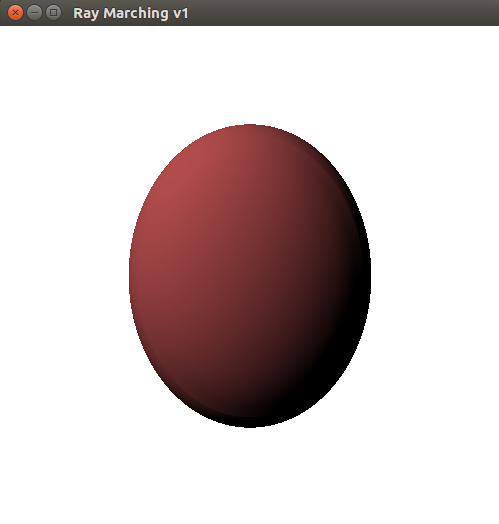
\includegraphics[width=0.8\textwidth]{imagenes/Prueba2.png}
	\end{center}
	\caption{Prueba de la implementación de Ray-Marching usando la ecuación implícita de un elipsoide.}
	\label{fig:etiq_10}
\end{figure}
${ }$\\

${ }$\\
\subsection{Otros ejemplos de ovaloides}
${ }$\\

En la clase $OvaloidePrueba$ se representa el ovaloide visto anteriormente de ecuación $x^4 + y^4 + z^4 = 1$, el resultado puede verse en la Figura \ref{fig:etiq_12}.
${ }$\\

\begin{lstlisting}[style=Consola]
class OvaloidePrueba : public Superficie{

private:


public :

	OvaloidePrueba(Tupla3f c);
	double funcion(Tupla3f xyz);
};

OvaloidePrueba::OvaloidePrueba(Tupla3f c):Superficie(c){

}

double OvaloidePrueba::funcion(Tupla3f xyz){

	return (pow(xyz.coo[0],4) + pow(xyz.coo[1],4) + pow(xyz.coo[2],4) -1);
}
\end{lstlisting}
${ }$\\

\begin{figure}[h]
	\begin{center}
		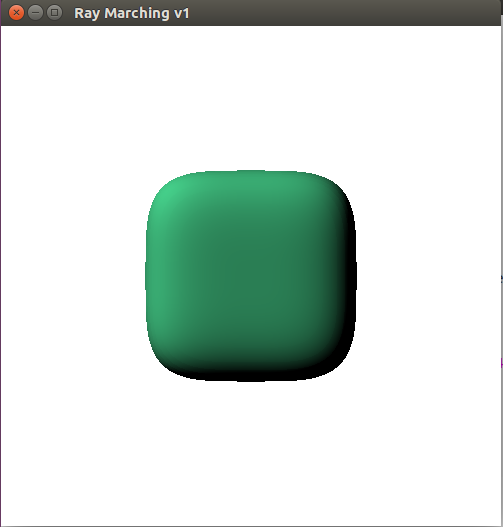
\includegraphics[width=0.8\textwidth]{imagenes/Ovaloid.png}
	\end{center}
	\caption{Ovaloide de ecuación $x^4 + y^4 + z^4 = 1$.}
	\label{fig:etiq_12}
\end{figure}
${ }$\\


${ }$\\
\subsection{Otras superficies.}
${ }$\\

También podemos visualizar otro tipo de superficies, por ejemplo cuádricas en la Figura se muestra la imagen de un hiperboloide.
${ }$\\

\begin{figure}[h]
	\begin{center}
		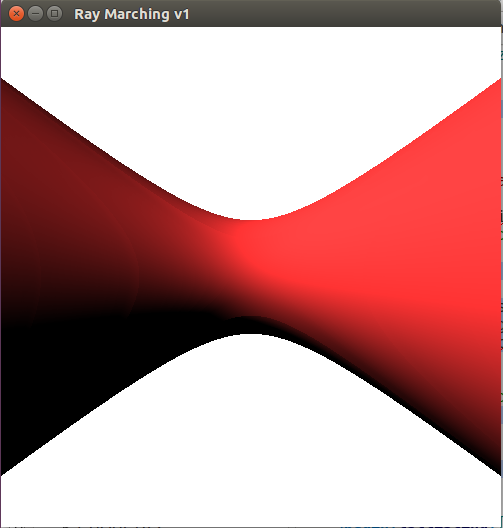
\includegraphics[width=0.8\textwidth]{imagenes/cuadrica.png}
	\end{center}
	\caption{Hiperboloide.}
	\label{fig:etiq_123}
\end{figure}


Superficies cuádricas tienen como ecuación implícita:
${ }$\\
\[
ax^2 + bxy + cxz +dx +ey^2 +fyz +gy + hz^2 + iz +j = 0.
\]
${ }$\\

El código para las cuádricas es el siguiente:
${ }$\\

\begin{lstlisting}[style=Consola]
class Cuadrica : public Superficie{

private:

	double a, b, c, d, e, f, g, h, i, j;

public :

	Cuadrica(double ac, double bc, double cc, double dc, double ec, double fc, double gc, double hc, double ic, double jc, Tupla3f c);
	double funcion(Tupla3f xyz);
};



Cuadrica::Cuadrica(double ac, double bc, double cc, double dc, double ec, double fc, double gc, double hc, double ic, double jc, Tupla3f col):Superficie(col){
	a = ac;
	b = bc;
	c = cc;
	d = dc;
	e = ec;
	f = fc;
	g = gc;
	h = hc;
	i = ic;
	j = jc;
}

double Cuadrica::funcion(Tupla3f xyz){

	return (a*pow(xyz.coo[0],2) + b*(xyz.coo[0]*xyz.coo[1]) + c*(xyz.coo[0]*xyz.coo[2]) +d*xyz.coo[0] +e*pow(xyz.coo[1],2) +f*(xyz.coo[1]*xyz.coo[2]) +g*xyz.coo[2] + h*pow(xyz.coo[2],2) + i*xyz.coo[2] +j);
}
\end{lstlisting}





